%!TEX root = LookingGlass.tex




%  Let $\Phi$ be a $m$-strongly convex function in $\norm{\cdot}$, define a projection operator $\Pi^\Phi_K : \mathbb{R}^n \rightarrow K$ as 
% \[
% \Pi^\Phi_K(u) = \arg\min_{v \in K} D_{\Phi}(v, u).
% \]

% The following online projection algorithm is the building block for this note. We show that, by choosing appropriate $l$ to balance between the movement costs, hit costs, and the gradient of hit costs, we can derive constant competitive algorithms in Section \ref{sec: alg-cr} and low dynamic regret algorithm in Section \ref{sec: alg-regret}.  
% \begin{algorithm}
% 	\begin{algorithmic}[1]
% 			\REQUIRE Starting point $x_0$, mirror map $\Phi$.
% 			\FOR{$t=1, \ldots, T$}
% 			\STATE Choose an appropriate sublevel set $K_l = \{ x \mid f_t(x) \le l\}$, \\
% 			  set $x_t = \Pi^{\Phi}_{K_l}(x_{t-1})$.
%               \label{alg: gradient-step}
% 			\ENDFOR
% 	\end{algorithmic}
% \caption{Online projection (meta algorithm)}
% \label{alg: online-projection}
% \end{algorithm}




% \subsection{Geometric intuition}
% Algorithm \ref{alg: online-projection} can be viewed as moving in a direction that is perpendicular to the level set as illustrated in Fig. \ref{fig: convex-geometry}. \niangjun{change this sentence as it no longer describes the geometric intuition now that we move to the mirror descent setting}
% % \begin{figure}
% % \centering
% % \includegraphics[width=.3\textwidth]{projection-step}
% % \caption{Illustration of one step of Algorithm \ref{alg: online-projection}, the algorithm chooses appropriate sublevel set $K_l = \{x \mid f_t(x) \le l\}$, and set $x_t = \Pi_{K_l}(x_{t-1})$.}
% % \label{fig: convex-geometry}
% % \end{figure}
% We have the following property that will be useful for proving our theoretical results \cite[Lemma 4.1]{bubeck2015}: 
% \begin{proposition}
% For $x_t, x_{t-1}, K_l$ in step \ref{alg: gradient-step} of Algorithm \ref{alg: online-projection}, for any $y \in K_l$, we have 
% \[
% 	D_{\Phi} (x_t , x_{t-1} ) + D_\Phi ( y, x_t )\le D_\Phi(y, x_{t-1}).
% \]
% \label{prop: convex-proj-ineq}
% \end{proposition} 
% When $\Phi$ is the 2-norm square $\norm{\cdot}^2$, $x_t$, $x_{t-1}$ and $y$ form an obtuse triangle. 

% Then we can write the $x_t$ as the solution of the following optimization problem for some $l$: 
% \begin{align*}
% \min & \quad D_{\Phi}(x, x_{t-1}) \\
% \text{s.t.}& \quad f_t(x) \le l.
% \end{align*}
% Let $\eta_t$ be the optimal dual variable for the inequality constraint that is dependent on $l$, by the first order optimality condition
% \begin{equation}
% \nabla \Phi(x_t) = \nabla \Phi(x_{t-1}) - \eta_t \nabla f_t (x_t).
% \label{eqn: mirror-descent-step}
% \end{equation}
% While \eqref{eqn: mirror-descent-step} looks similar to a step in online mirror descent, it is not the same since the update direction in the ``dual space'' is in the one-step future gradient $\nabla f_t(x_t)$ instead of the current gradient $\nabla f_{t-1}(x_{t-1})$. 

% Let $I_C$ be the indicator function. Table \ref{table: algorithm-comparison} summarizes the main differences between $\ouralg$ with online gradient descent (OGD) and online mirror descent (OMD). 
% \begin{table}[tbh]
% \centering
% \begin{tabular}{|c|l|}
% \hline 
% Algorithm & Update rule\\
% \hline 
% OGD & $ x_t = \argmin_{x \in \mathcal{X}} \eta_t \langle x, \nabla f_{t-1}(x_{t-1}) \rangle + \frac{1}{2} \norm{x - x_{t-1}}^2 $ \\
% \hline
% \ouralg, GD version & $ x_t = \argmin_{x } I_C(\{ x | f(x) \le l \}) + \frac{1}{2} \norm{x - x_{t-1}}^2 $ \\
% \hline
% OMD & $ x_t = \argmin_{x \in \mathcal{X}} \eta_t \langle x, \nabla f_{t-1}(x_{t-1}) \rangle + D_{\Phi}(x, x_{t-1}) $ \\
% \hline
% \ouralg, MD version & $ x_t = \argmin_{x} I_C(\{ x | f(x) \le l \}) + D_{\Phi}(x, x_{t-1}) $ \\
% \hline
% \end{tabular}
% \caption{Comparison between online gradient descent (OGD), online mirror descent (OMD), and two versions of our proposed algorithm. The step size of OGD and OMD is controlled by $\eta_t$, while the step size of $\ouralg$ is indirectly controlled by $l$.}
% \label{table: algorithm-comparison}
% \end{table}
% Note that while OGD and OMD can directly control the step size $\eta_t$, $ouralg$ need to control the step size indirectly via setting appropriate value of $l$. Furthermore, we set $l$ in order to achieve balance between the movement cost, hit cost, and the size of the gradient. We show how this can be done in the next two sections.  

% \begin{example}[Ball setup]
% When the norm is the Euclidean norm $\norm{\cdot}_2$, we can use $\Phi(x) = \frac{1}{2} \norm{x}_2^2$ as the mirror map, which is strongly convex in the Euclidean norm, in this case, the Bregman divergence is $D_\Phi(x, y) = \frac{1}{2} \norm{x - y}^2$, the update rule can be viewed as 
% \[ x_t = x_{t-1} - \eta_t \nabla f_t(x_t),
% \] for some $\eta_t$ controlled by $l$.  
% \end{example}

% \begin{example}[Simplex setup]
% When the feasible set is the simplex $\Delta = \{ x | \sum_{i=1}^n x_i = 1, x_i \ge 0, \forall i\}$ and the norm is the $l_1$-norm $\norm{\cdot}_1$, we can use the negative entropy $\Phi(x) = \sum_{i=1}^n x_i \log x_i$ as the mirror map since it is strongly convex in $\norm{\cdot}_1$ (by Pinsker's inequality).  In this case, the Bregman divergence  is given by $D_\Phi(x ,y) = \sum_{i=1}^n x_i \log\left( \frac{x_i}{y_i}\right)$ (also known as the Kullback-Leibler divergence), the update rule can be viewed as 
% \[
% x_t = \frac{1}{\norm{x_t}}_1 x_{t-1}e^{-\eta_t \nabla f_t(x_t)},
% \]
% for some $\eta_t$ controlled by $l$.
% \end{example}


% \begin{example}[Spectrahedron setup]
% When the feasible set is the set of positive semidefinite matrices with trace 1 and the norm is the Schatten-1 norm, we can use the negative von-Neumann entropy as the mirror map: $ \Phi(X) = \sum_{i=1}^n \lambda_i(X)\log \lambda_i(X)$, where $\lambda_i(X)$ is the $i$-th eigenvalue of $X$. We can show that $\Phi$ is strongly convex in the Schatten 1-norm. In this case, the update rule can be viewed as 
% \[
%   X_{t} = \exp (\log X_{t-1} - \eta_t \nabla f_t(X_t)),
% \]
% for some $\eta_t$ controlled by $l$. 
% \end{example}


% %
% %The following online projection algorithm is the building block for this note. We show that, by choosing appropriate $l$ to balance between the movement costs, hit costs, and the gradient of hit costs, we can derive constant competitive algorithms in Section \ref{sec: alg-cr} and low dynamic regret algorithm in Section \ref{sec: alg-regret}.  
% %\begin{algorithm}
% %	\begin{algorithmic}[1]
% %			\FOR{$t=1, \ldots, T$}
% %			\STATE Choose an appropriate sublevel set $K_l = \{ x \mid f_t(x) \le l\}$, \\
% %			  set $x_t = \Pi_{K_l}(x_{t-1})$.
% %              \label{alg: gradient-step}
% %			\ENDFOR
% %	\end{algorithmic}
% %\caption{Online projection (meta algorithm)}
% %\label{alg: online-projection}
% %\end{algorithm}

% %\subsection{Geometric intuition}
% %Algorithm \ref{alg: online-projection} can be viewed as moving in a direction that is perpendicular to the level set as illustrated in Fig. \ref{fig: convex-geometry}. 
% %\begin{figure}
% %\centering
% %\includegraphics[width=.3\textwidth]{projection-step}
% %\caption{Illustration of one step of Algorithm \ref{alg: online-projection}, the algorithm chooses appropriate sublevel set $K_l = \{x \mid f_t(x) \le l\}$, and set $x_t = \Pi_{K_l}(x_{t-1})$.}
% %\label{fig: convex-geometry}
% %\end{figure}
% %We have the following property that will be useful for proving our theoretical results \cite[Lemma 3.1]{bubeck2015}: 
% %\begin{proposition}
% %For $x_t, x_{t-1}, K_l$ in step \ref{alg: gradient-step} of Algorithm \ref{alg: online-projection}, for any $y \in K_l$, we have 
% %\[
% %	\norm{x_{t-1} - x_t}^2 + \norm{x_t - y}^2 \le \norm{x_{t-1} - y}^2,
% %\]
% %i.e., the points $x_{t-1}$, $x_t$ and $y$ form an obtuse triangle. 
% %\label{prop: convex-proj-ineq}
% %\end{proposition} 
% %
% %
% %\subsection{Comparison with gradient descent and mirror descent}
% %Since we are moving in a direction that is perpendicular to the level set, we can view Algorithm \ref{alg: online-projection} as a gradient update. Formally, we can write $x_t$ as the solution of the following optimization problem for some $l$:
% %\begin{align*}
% %\min_x & \quad \frac{1}{2} \norm{x_{t-1} - x}_2^2 \\
% %\text{s.t.} & \quad f_t(x) \le l.
% %\end{align*} 
% %Let $\eta_t \ge 0$ be the optimal Lagrange multiplier of the inequality constraint, then 
% %% the Lagrangian 
% %% \[ L(x, \lambda) = \frac{1}{2} \norm{x_{t-1} - x}_2^2 + \lambda (f_t(x) - l) ,\]
% %by the KKT condition $\partial_x L = 0$ 
% %%when $x = x_t$ and $\lambda = \lambda^*$, 
% %we have 
% %% \begin{equation}
% %% 	 x_{t-1} - x_t = \eta_t \nabla f_t(x_t)
% %% 	\label{eqn: gradient-update}
% %% \end{equation}
% %%From \eqref{eqn: gradient-update} we can see that, $x_{t-1} - x_t$ is parallel to the gradient of $f_t$ at $x_t$. 
% %%Hence we can write the update rule as 
% %\begin{equation}
% %	 x_t = x_{t-1} - \eta_t \nabla f_t(x_t),
% %	\label{eqn: gradient-step}
% %\end{equation}
% %for some $\eta_t$ dependent on $l$. 
% % However, instead of moving in the direction of the current gradient, Algorithm \ref{alg: online-projection} is moving in the direction of the one step future gradient $\nabla f_t(x_t)$. Hence while \eqref{eqn: gradient-step} looks similar to online gradient descent, it can not be directly implemented as $x_t$ appears on both side of the equation.  
% %
% %For switching cost in any other norm $\norm{\cdot}_a$, we can define projection using Bregman divergence for some mirror map $\Phi$. 
% %\begin{definition}
% %The Bregman divergence $D_\phi$ for a convex function $\phi$ is defined by 
% %\[D_{\phi}(x, y) = \phi(x) -\phi(y) - \nabla\phi(y)^T(x-y). \]
% %\end{definition}
% %Let $\Phi : \mathcal{X} \rightarrow \mathbb{R}$ be a strongly convex function in $\norm{\cdot}_a$, and $\nabla \Phi(\mathcal{X}) = \mathbb{R}^n$. Since the function $x \rightarrow \frac{1}{2} \norm{x}^2$ is a natural mirror map for the Euclidean norm. We can think of this as a generalization of the online projection. Define projection $\Pi_K(u) = \argmin_{v \in K} D_{\Phi}(v, u).$ Then we can write the $x_t$ as the solution of the following optimization problem for some $l$: 
% %
% %\begin{align*}
% %\min & \quad D_{\Phi}(x, x_{t-1}) \\
% %\text{s.t.}& \quad f_t(x) \le l.
% %\end{align*}
% %Let $\eta_t$ be the optimal dual variable for the inequality constraint that is dependent on $l$, by the first order optimality condition
% %\begin{equation}
% %\nabla \Phi(x_t) = \nabla \Phi(x_{t-1}) - \eta_t \nabla f_t (x_t).
% %\label{eqn: mirror-descent-step}
% %\end{equation}
% %While \eqref{eqn: mirror-descent-step} looks similar to a step in online mirror descent, it is not the same since the update direction in the ``dual space'' is in the one-step future gradient $\nabla f_t(x_t)$ instead of the current gradient $\nabla f_{t-1}(x_{t-1})$. 
% %
% %Let $I_C$ be the indicator function. Table \ref{table: algorithm-comparison} summarizes the main differences between $\ouralg$ with online gradient descent (OGD) and online mirror descent (OMD). 
% %\begin{table}[tbh]
% %\centering
% %\begin{tabular}{|c|l|}
% %\hline 
% %Algorithm & Update rule\\
% %\hline 
% %OGD & $ x_t = \argmin_{x \in \mathcal{X}} \eta_t \langle x, \nabla f_{t-1}(x_{t-1}) \rangle + \frac{1}{2} \norm{x - x_{t-1}}^2 $ \\
% %\hline
% %\ouralg, GD version & $ x_t = \argmin_{x } I_C(\{ x | f(x) \le l \}) + \frac{1}{2} \norm{x - x_{t-1}}^2 $ \\
% %\hline
% %OMD & $ x_t = \argmin_{x \in \mathcal{X}} \eta_t \langle x, \nabla f_{t-1}(x_{t-1}) \rangle + D_{\Phi}(x, x_{t-1}) $ \\
% %\hline
% %\ouralg, MD version & $ x_t = \argmin_{x} I_C(\{ x | f(x) \le l \}) + D_{\Phi}(x, x_{t-1}) $ \\
% %\hline
% %\end{tabular}
% %\caption{Comparison between online gradient descent (OGD), online mirror descent (OMD), and two versions of our proposed algorithm. The step size of OGD and OMD is controlled by $\eta_t$, while the step size of $\ouralg$ is indirectly controlled by $l$.}
% %\label{table: algorithm-comparison}
% %\end{table}
% %Note that while OGD and OMD can directly control the step size $\eta_t$, $ouralg$ need to control the step size indirectly via setting appropriate value of $l$. Furthermore, we set $l$ in order to achieve balance between the movement cost, hit cost, and the size of the gradient. We show how this can be done in the next two sections.  

% \subsection{Balancing between the movement cost and the hit cost}
% \label{sec: balance-movement-hit}
% The key idea of choosing $K_l$ in step \ref{alg: gradient-step} of Algorithm \ref{alg: online-projection} is to strike balance between movement cost and hit cost (or size of the gradient). Here we show that this can be efficiently done by the following Lemma. Note that the hit cost $f_t(x_t) = l$, and the movement cost $\norm{x_t - x_{t-1}} = d(x_{t-1}, K_l)$ where we define the distance from a point to a convex set $d(u, K) = \min_{v \in K} \norm{u-v}$. 
% %\begin{lemma}
% %		The function $g(l) = d(x_{t-1}, K_l)$ is convex and decreasing in $l$. 
% %		\label{lem: convexity-distance}
% %\end{lemma}

% \begin{lemma}
% 		Let $x(l) = \argmin_{K_l} D_{\Phi}(x, x_{t-1}) $. The function $g(l) = \norm{x(l) - x_{t-1}}$ is continuous in $l$. 
% 		\label{lem: continuity-distance}
% \end{lemma}

% Given Lemma \ref{lem: continuity-distance}, let $l_0 = f_t(v_t)$, and $l_1 = f_t(x_{t-1})$,  we know that $ g(l_0) > \beta l_0 $, and $0 = g(l_1) < \beta l_1$. By intermediate value theorem, there exists $l_0 < l < l_1$ such that $ g(l) = \beta l$, i.e., $\norm{x_t - x_{t-1}} = \beta f_t(x_t)$.


% Further, by continuity of the function  $ g(l) - \beta l$, we can use bisection to find $l$ such that $g(l) = \beta l$. Computing the projection $\Pi_{K_l}(x_{t-1})$ for each individual $l$ is a convex problem, hence we can compute step \ref{projection-step-cr} in polynomial time independent of $T$.

% %Since convex functions are continuous, given this Lemma, let $l_0 = f_t(v_t)$, and $l_1 = f_t(x_{t-1})$,  we know that $ g(l_0) > \beta l_0 $, and $0 = g(l_1) < \beta l_1$. By intermediate value theorem, there exists $l_0 < l < l_1$ such that $ g(l) = \beta l$, i.e., $\norm{x_t - x_{t-1}} = \beta f_t(x_t)$
% %
% %Further, note that $ g(l) - \beta l$ is a monotonically decreasing function, we can use bisection to find $l$. Furthermore, computing $d(x_{t-1}, K_l)$ for each individual $l$ is a convex problem, hence we can compute $l$ that achieve the desired balance in polynomial time independent of $T$.


% %We show in this section that we can balance between the movement cost and the hit cost by choosing the sublevel set $K_l$ in an efficient manner. In Section \ref{sec: alg-cr} we show that balancing the movement cost and the hit cost lead to a constant competitive algorithm that is dimension free.


% \subsection{Balancing between the movement cost and the size of the gradient}
% \label{sec: balance-movement-grad}
% In this section we show that we can choose $l$ to balance between the movement cost $\norm{x_t - x_{t-1}}$ and the size of the gradient $\norm{\nabla f_t(x_t)}$, which can be view as a ``marginal cost'', we claim that this step is well-defined and computationally efficient by the following Lemma: 
% \begin{lemma}
% The function $h(l) = \frac{\norm{x_{t-1} - x_l }}{\norm{\nabla{f_t(x_l)}}}$ is a continuous and decreasing function in $l$. 
% \label{lem: continuity-ratio}
% \end{lemma}


% Given Lemma \ref{lem: continuity-ratio}, by continuity of $h(l)$, there exists an $l$ such that $h(l) = \eta$, and by monotonicity of $h(l)$, we can find such $l$ efficiently via bisection to complete Step \ref{projection-step-regret}. We show in this section that we can balance between the movement cost and the size of gradient by choosing the sublevel set $K_l$ in an efficient manner. In Section \ref{sec: alg-regret} we show that this will lead to an online algorithm with low dynamic regret.





%  let $\kappa = \frac{M}{m}$ be the condition number of $\Phi$. Define a projection operator $\Pi^\Phi_K : \mathbb{R}^n \rightarrow K$ as 
% \[
% \Pi^\Phi_K(u) = \arg\min_{v \in K} D_{\Phi}(v, u).
% \]


The core of this paper is a new algorithmic framework for online convex optimization that we term \emph{\ouralg} (\ourack). \ourack\ represents the first algorithmic framework that applies to both competitive analysis and regret analysis in SOCO problems and, as such, parallels recent results that have begun to provide unified algorithmic techniques for competitiveness and regret in other areas.  For example,  \cite{buchbinder2012unified} and \cite{Blum2000} provided frameworks that bridged competitiveness and regret in the context of MTS problems, which have a discrete action spaces, and \cite{blum2002static} did the same for decision making problems on trees and lists. 

\ourack\ builds both on ideas from online algorithms, specifically the work of \cite{bansal2015}, and online learning, specifically Online Mirror Descent (OMD) \citep{nemirovskii1983problem, warmuth1997continuous, bubeck2015}.  We begin this section with the geometric intuition underlying the design of \ourack\ in Section \ref{sec:alg-geometry}.  Then, in Section \ref{sec:alg-description}, we describe the details of the algorithm. Finally, in Section \ref{sec:alg-examples} we provide illustration of how the choice of the mirror map impacts the behavior of the algorithm. 

\subsection{A Geometric Interpretation}
\label{sec:alg-geometry}

%A classical approach for online optimization is to move greedily towards the minimizer $v_t$ during each round \niangjun{OGD doesn't move towards $v_t$ as well}.  Assuming this structure, the only design choice left is how to pick the step-size at each round. In contrast, 
The key insight that drives the design of \ourack\ is that it is the geometry of the level sets, not the location of the minimizer, which should guide the choice of $x_t$. %To see this, consider a cost function whose level sets are elongated ellipses. Suppose the previous point $x_{t-1}$ is located near the end of such an ellipse. Moving directly towards the minimizer incurs an unnecessarily high switching cost; a much cheaper action would be to be \emph{lazy} and simply project onto the level set. This incurs the same hitting cost, but much less switching cost. 
This reasoning leads naturally to an algorithm for SOCO that, at each round, projects the previous point $x_{t-1}$ onto a level of the current cost function $f_t$. However, the question of ``which level set?'' remains.  This choice is where the name \ouralg\ comes from -- \ourack\ chooses a level set that \emph{balances} the switching cost and hitting costs, where the notion of balance used is the heart of the algorithm.  

To make the intuition described above more concrete, assume for the moment that the switching cost is defined by the $\ell_2$ norm. Suppose the algorithm has decided to project onto the $l$-level set of $f_t$ (we show how to pick $l$ in the next section). Then the action of the algorithm is the solution of the following optimization problem: 
%
\begin{align*}
\text{minimize} \quad \frac{1}{2}\norm{x - x_{t-1}}^2 \qquad \text{subject to } \quad f_t(x) \le l.
\end{align*}
%
Now, let $\eta_t$ be the optimal dual variable for the inequality constraint. By the first order optimality condition, $x_t$ needs to satisfy 
$$x_t = x_{t-1} - \eta_t \nabla f_t(x_t).$$
This resembles a step of Online Gradient Descent (OGD), except that the update direction is the gradient $\nabla f_t(x_t)$ instead of $\nabla f_{t-1}(x_{t-1})$, and the step size $\eta_t$ is allowed to vary. Hence in this setting \ourack\ can be seen as a ``one step ahead'' version of OGD with time-varying step sizes.

\begin{figure}[t]
\floatconts
  {fig:subfigex}
  {\caption{\textit{An illustration of the difference between \ourack\ and OMD assuming the mirror map $\Phi(x) = \frac{1}{2}\norm{x}^2_2$. While OMD steps in a direction normal to the contour line of $f_{t-1}(\cdot)$ at $x_{t-1}$, \ourack\  steps in a direction normal to the contour line of $f_t(\cdot)$ at $x_t$. }}
  \label{fig: comparison}}
  {%
    \subfigure[\textit{A step taken by OMD. Contour lines represent the sub-level sets of $f_{t-1}$.}]{\label{fig: omd_step}%
      \hspace{.5in} 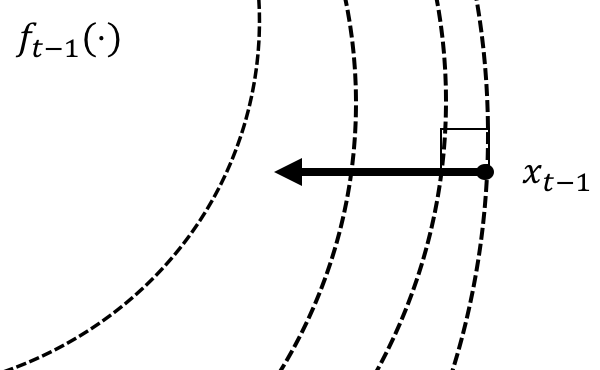
\includegraphics[width=0.23\linewidth]{comparison_5a}\hspace{.5in}}%
    \qquad \quad
    \subfigure[\textit{A step taken by \ourack. Contour lines represent the sub-level sets of $f_{t}$.}]{\label{fig: ouralg_step}%
      \hspace{.5in}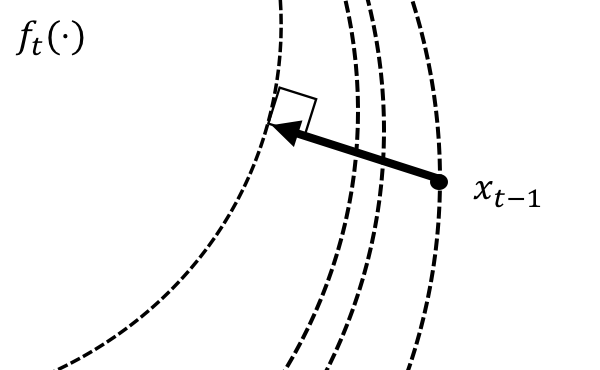
\includegraphics[width=0.23\linewidth]{comparison_5b}\hspace{.5in}}
 \vspace{-.2in}
 }
 \vspace{-.15in}
\end{figure}

For more general switching costs a similar geometric intuition can be obtained using a mirror map $\Phi$ with respect to the norm $\| \cdot \|$.  Here, $x_t$ is the solution of the following optimization in dual space where, given a convex function $\Phi$, $D_\Phi(x, y)$ is the Bregman divergence between $x$ and $y$, i.e., $D_\Phi(x, y) = \Phi(x) - \Phi(y) - \nabla \Phi(y)^T(x-y)$: 
\begin{align*}
\text{minimize}  \quad D_{\Phi}(x, x_{t-1}) \qquad
\text{subject to} \quad f_t(x) \le l.
\end{align*}
As before, let $\eta_t$ be the optimal dual variable for the inequality constraint. The first order optimality condition implies that $x_t$ must satisfy 
\begin{equation}
\nabla \Phi(x_t) = \nabla \Phi(x_{t-1}) - \eta_t \nabla f_t (x_t).
\label{eqn: mirror-descent-step}
\end{equation}
The form of \eqref{eqn: mirror-descent-step} is similar to a ``one step ahead'' version of OMD with time varying $\eta_t$, i.e., the update direction in the dual space is in the gradient $\nabla f_t(x_t)$ instead of the gradient $\nabla f_{t-1}(x_{t-1})$. The implicit form of the update has been widely used in online learning, e.g., \cite{kivinen1997exponentiated, kulis2010implicit}.

Figure \ref{fig: comparison} illustrates the difference between \ourack\ and OMD when $\Phi(x) = \frac{1}{2}\norm{x}^2_2$: \ourack\ is normal to the destination whereas OMD is normal to the starting point. Intuitively, this is why the guarantees we obtain for \ourack\ are stronger than what previous descent-based approaches have obtained in this setting -- it is better to move in the direction determined by the level set where you land, than the direction determined by the level set where you start. 

\subsection{A Meta Algorithm}
\label{sec:alg-description}

The previous section gives intuition about one key aspect of the algorithm, the projection onto a level-set.  But, in the discussion above we assume we are projecting onto a specific $l$-sublevel set. The core of \ourack\ is that this sublevel set is determined endogenously in order to ``balance'' the switching and hitting costs, as opposed to a fixed exogenous schedule of step-sizes like is typical in many online descent algorithms. Informally, the operation of \ourack\ is summarized in the \emph{meta algorithm} in Algorithm \ref{alg: online-projection}, which uses the operator $\Pi^\Phi_K(x) : \mathbb{R}^n \rightarrow K$ to denote the Bregman projection of $x$ onto a convex set $K$, i.e., $\Pi^\Phi_K(x) = \argmin_{y \in K} D_\Phi(y, x)$, where $\Phi$ is $m$-strongly convex and $M$-Lipschitz smooth in $\norm{\cdot}$, i.e., $ \frac{m}{2} \norm{x-y}^2 \le D_\Phi(x,y) \le \frac{M}{2} \norm{x-y}^2.$



We term Algorithm \ref{alg: online-projection} a meta algorithm because the general framework given in Algorithm \ref{alg: online-projection} can be instantiated with different forms of ``balance'' in order to perform well for different metrics.  More specifically, the notion of ``balance'' in the Step \ref{alg:meta-balance} that is appropriate varies depending on whether the goal is to perform well for competitive ratio or for regret.  

Our results in this paper highlight two different approaches for defining \emph{balance} in \ourack\ based on either balancing the switching cost with the hitting cost in either the primal or dual space.  We  balance costs in the primal space to yield a constant, dimension-free competitive algorithm for locally polyhedral cost functions (Section \ref{sec: alg-cr}), and balance in the dual space to yield a no-regret algorithm (Section \ref{sec: alg-regret}). We summarize these two approaches in the following and then give more complete descriptions in the corresponding technical sections.  

%\adam{Need to reincorporate the following: Let $x(l) = \Pi^\Phi_{K_l}(x_{t-1})$.  }

\begin{algorithm}[t]
	\begin{algorithmic}[1]
			\REQUIRE Starting point $x_0$, mirror map $\Phi$.
			\FOR{$t=1, \ldots, T$}
			\STATE Choose a sublevel set $K_l = \{ x \mid f_t(x) \le l\}$ to ``balance'' the switching and hitting costs.  \label{alg:meta-balance}
			  \STATE Set $x_t = \Pi^{\Phi}_{K_l}(x_{t-1})$.
              \label{alg: gradient-step}
			\ENDFOR
	\end{algorithmic}
\caption{\ouralg\ (\ourack), Meta Algorithm}
\label{alg: online-projection}
\end{algorithm}

\begin{itemize}
\item{\textbf{Primal \ouralg}}.  The algorithm we consider in Section \ref{sec: alg-cr} instantiates Algorithm \ref{alg: online-projection} by choosing $l$ such that $x(l) = \Pi^\Phi_{K_l}(x_{t-1})$ achieves balance between the switching cost with the hitting cost in the \emph{primal} space. Specifically, for some fixed $\beta>0$, choose $l$ such that either $x(l) = \argmin_x f_t(x)$ and $\norm{x(l) - x_{t-1}} < \beta l $, or the following is satisfied:
\begin{equation}
\norm{x(l) - x_{t-1}} = \beta l
\label{eqn: primal-balance}
\end{equation}

\item{\textbf{Dual \ouralg}}. The algorithm we consider in Section \ref{sec: alg-regret} instantiates Algorithm \ref{alg: online-projection} by balancing the switching cost with the size of the gradient in the \emph{dual} space.  Specifically, for some fixed $\eta$, we choose $l$ such that 
\begin{equation}
\norm{\nabla \Phi(x(l)) - \nabla \Phi(x_{t-1})}_* = \eta \norm{\nabla f_t(x(l))}_*,
\label{eqn: dual-balance}
\end{equation}
\end{itemize}

The final piece of the algorithm is computational.  Note that the algorithm is \emph{memoryless}, i.e., it does not use any information about previous cost functions.  Thus, the only question about efficiency is whether the appropriate $l$ can be found efficiently.  The following lemmas verify that, indeed, it is possible to compute $l$, and thus implement \ourack, efficiently.  

\begin{lemma}
		The function $g(l) = \norm{x(l) - x_{t-1}}$ is continuous in $l$. 
		\label{lem: continuity-distance}
\end{lemma}

\begin{lemma}
Consider $\Phi$ and $f_t$ that are continuously differentiable on $\mathcal{X}$. The function \\ $h(l) = \frac{\norm{\nabla \Phi(x_{t-1}) - \nabla \Phi(x(l)) }_*}{\norm{\nabla{f_t(x(l))}}_*}$ is continuous in $l$. 
\label{lem: continuity-ratio}
\end{lemma}

The continuity of $g(l)$ and $h(l)$ in $l$ is enough to guarantee efficient implementation of Primal and Dual \ourack\ because it shows that an $l$ satisfying the balance conditions in the algorithms exists and, further, can be found to arbitrary precision via bisection.  Proofs are included in the appendix.

\subsection{Examples}
\label{sec:alg-examples}

An important part of the design of an \ourack\ algorithm is the choice of the mirror map.  
%Recall that \ourack\ needs to choose a mirror map that is both strongly convex and Lipschitz smooth for the norm defined by the switching cost. Clearly, 
Different choices of a mirror map $\Phi$ can lead to very different behavior by the resulting algorithms. To highlight this, and give intuition for the impact of the choice, we describe three examples of mirror maps below.  These examples focus on mirror maps that are commonly used for OMD, and they highlight interesting connections between the \ourack\ framework and classical online optimization algorithms like OGD \citep{zinkevich2003} and Multiplicative Weights \citep{arora2012}.

\paragraph{Euclidean norm squared:} Consider $\Phi(x) = \frac{1}{2}\norm{x}_2^2$, which is both 1-strongly convex and 1-Lipschitz smooth for the $\ell_2$ norm. Note that $\nabla \Phi(x) = x$.  Then, the first order condition \eqref{eqn: mirror-descent-step} is 
\begin{equation}
x_t = x_{t-1} - \eta_t \nabla f_t(x_t).
\label{eqn: one-step-ahead-GD}
\end{equation}
Interestingly, this can be interpreted as a ``one-step ahead'' OGD (illustrated in Figure \ref{fig: comparison}).  However, note that this equation should not be interpreted as an update rule since $x_t$ appears on both side of the equation.  In fact, this contrast highlights an important difference between OGD and \ourack.

\paragraph{Mahalanobis distance square:} Consider $\Phi(x) = \frac{1}{2} \norm{x}_Q^2$ for positive definite definite $Q$, which is 1-strongly convex and 1-Lipschitz smooth in the Mahalanobis distance $\norm{\cdot}_Q$.  Note that $\nabla \Phi(x) = Qx$.  Then, the first order condition \eqref{eqn: mirror-descent-step} is 
\begin{equation}
x_t = x_{t-1} - \eta_t Q^{-1} \nabla f_t(x_t).
\label{eqn: one-step-ahead-weighted-GD}
\end{equation}
This is analogous to a ``one step ahead" OGD where the underlying metric is a weighted $\ell_2$ metric.

\paragraph{Negative entropy:} If the feasible set is the $\delta$-interior of the simplex $\mathcal{X} = P_\delta = \{ x \mid \sum_{i=1}^n x_i = 1, x_i \ge \delta\}$, and the norm is the $\ell_1$ norm $\norm{\cdot}$, the mirror map defined by the negative entropy $\Phi(x) = \sum_{i=1}^n x_i \log x_i$ is $\frac{1}{2\ln 2}$-strongly convex (by Pinsker's inequality) and $ \frac{1}{\delta \ln 2}$-Lipschitz smooth (by reverse Pinsker's inequality \citep{sason2015}). In this case, $\nabla \Phi(x) = \log x + 1_d$, where $1_d$ represents the all 1s vector in $\mathbb{R}^d$. Then, the first order condition is 
\begin{equation}
x_t =  x_{t-1}\exp(-\eta_t \nabla f_t(x_t)).
\label{eqn: one-step-ahead-multiplicative-weight}
\end{equation}
This can be viewed as a ``one-step ahead'' version of the multiplicative weights update. Again, this equation should not be interpreted as an update rule since $x_t$ appears on both side of the equation.




